
\documentclass[border=10pt, 12pt]{standalone}
\usepackage[svgnames]{xcolor}
\usepackage{amsmath}
\usepackage{pgfplots}
\pgfplotsset{compat=newest}
\usepackage[sfdefault]{FiraSans}
\usepackage{FiraMono}
\renewcommand*\familydefault{\sfdefault}
\begin{document}
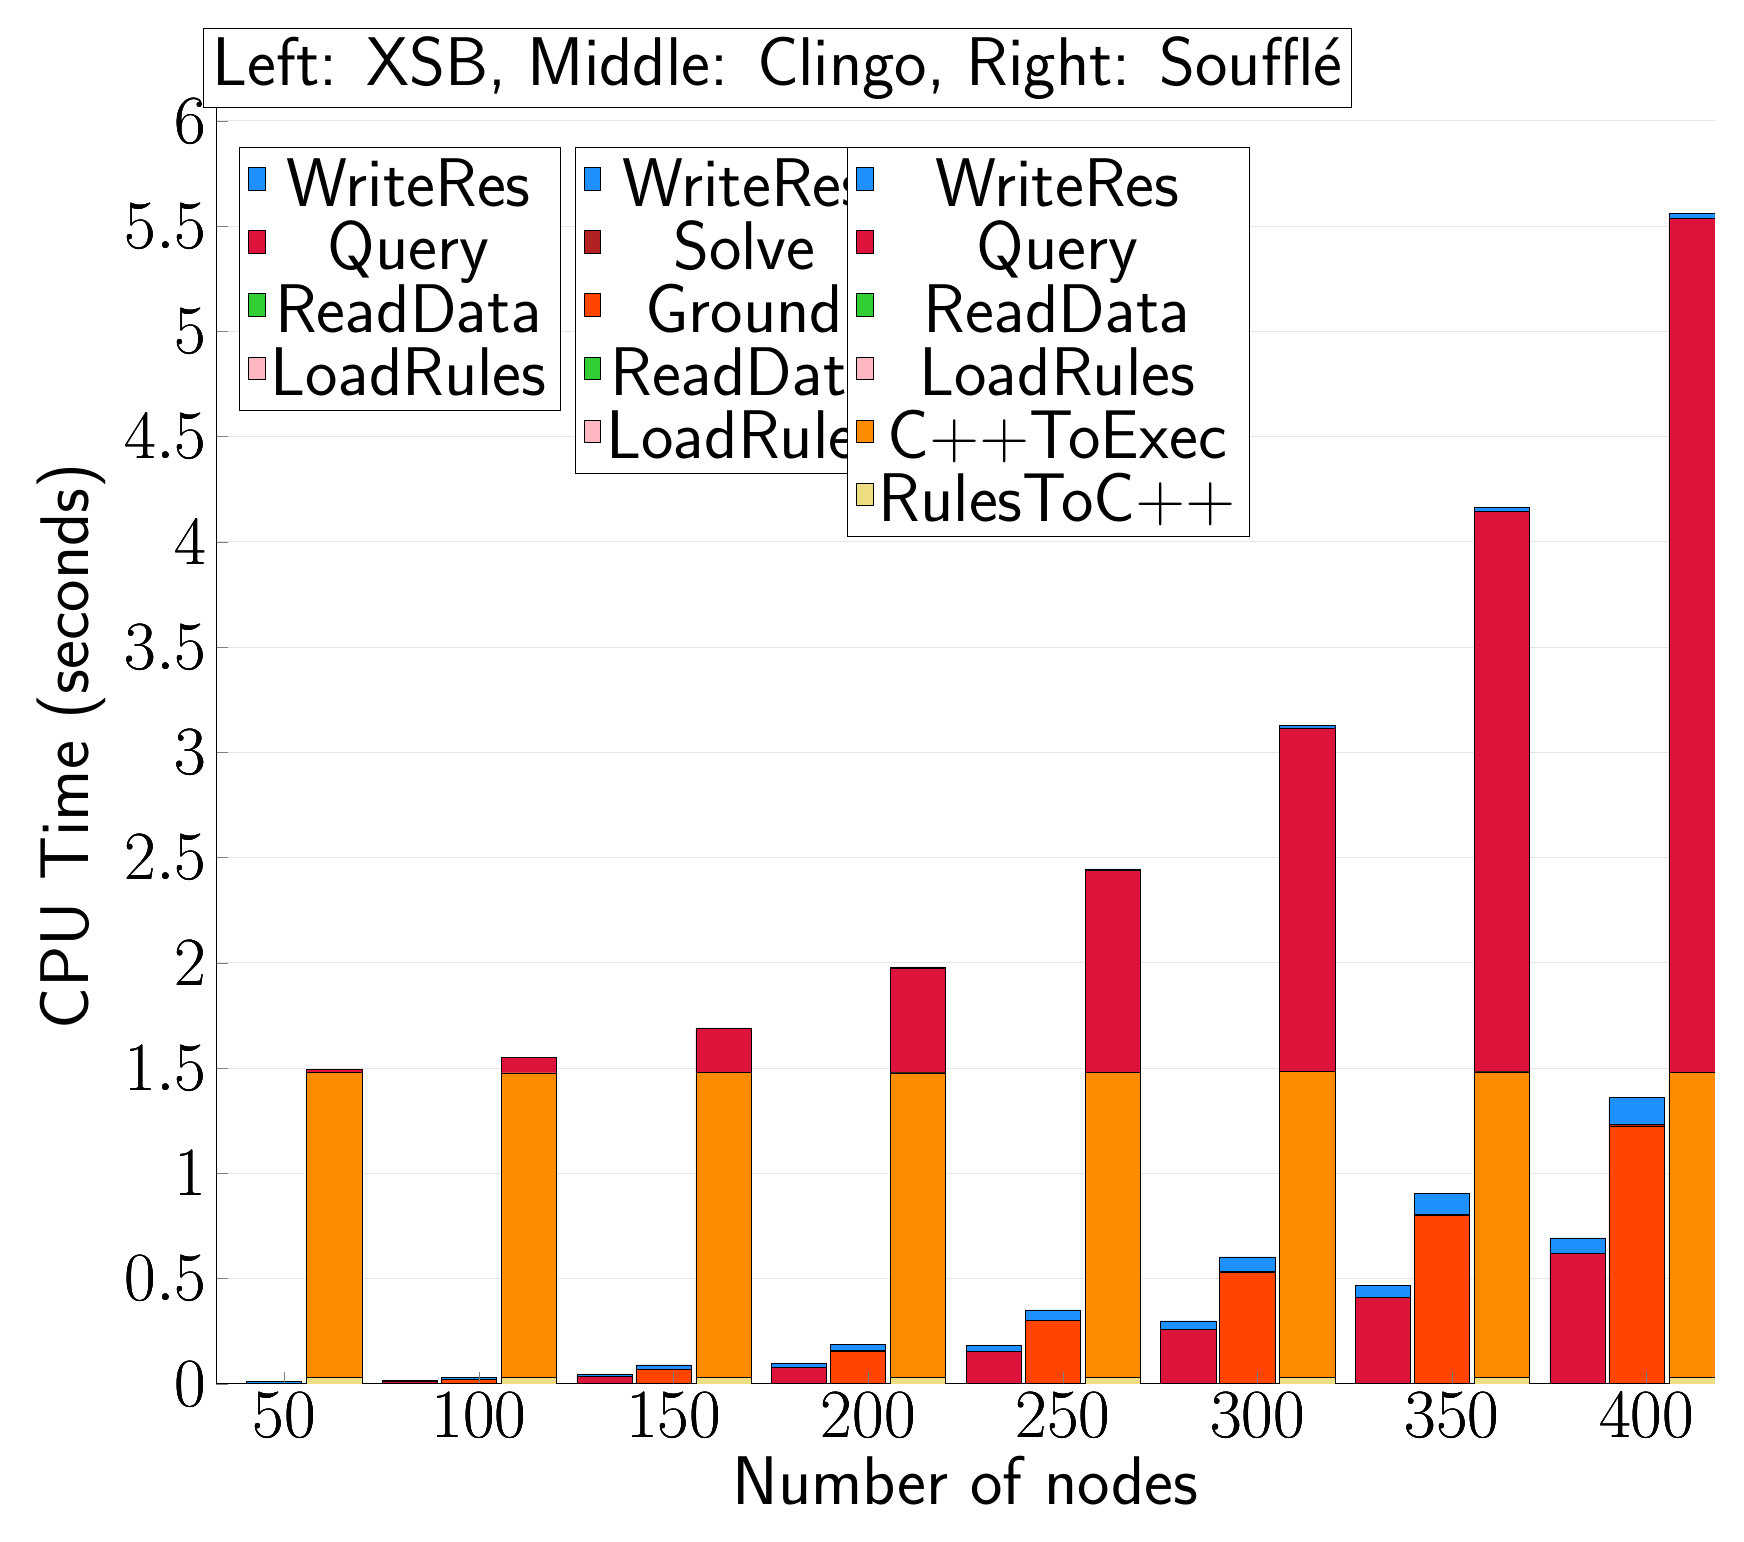
\begin{tikzpicture}
	\begin{axis}[bar shift=-25pt,
			ybar stacked,
			width=1.7\textwidth,
			bar width=0.7cm,
			ymajorgrids, tick align=inside,
			major grid style={draw=gray!20},
			xtick=data,
			ymin=0, ymax=6.059334,
			axis x line*=bottom,
			axis y line*=left,
			enlarge x limits=0.05,
			legend style={
					at={(0.23, 0.97)},
					anchor=north east,
					legend columns=1,
					font=\Huge,
				},
			ylabel={CPU Time (seconds)},
			xlabel={Number of nodes},
			label style={font=\Huge},
			tick label style={font=\Huge},
		]
		\addlegendimage{fill=DodgerBlue, draw=black, line width=0.2pt}
		\addlegendentry{WriteRes}
		\addlegendimage{fill=Crimson, draw=black, line width=0.2pt}
		\addlegendentry{Query}
		\addlegendimage{fill=LimeGreen, draw=black, line width=0.2pt}
		\addlegendentry{ReadData}
		\addlegendimage{fill=LightPink, draw=black, line width=0.2pt}
		\addlegendentry{LoadRules}
		\addplot +[fill=LightPink, draw=black, line width=0.2pt] coordinates {
				(50, 0.0005971999999999998)
				(100, 0.0006169999999999998)
				(150, 0.0005948000000000001)
				(200, 0.0006047000000000003)
				(250, 0.0006054000000000003)
				(300, 0.0006120000000000003)
				(350, 0.0006151000000000002)
				(400, 0.0006180000000000001)
			};
		\addplot +[fill=LimeGreen, draw=black, line width=0.2pt] coordinates {
				(50, 0.0001718)
				(100, 0.0002208)
				(150, 0.0002559000000000001)
				(200, 0.00030809999999999985)
				(250, 0.00034659999999999997)
				(300, 0.00039219999999999994)
				(350, 0.00043989999999999947)
				(400, 0.0004864999999999994)
			};
		\addplot +[fill=Crimson, draw=black, line width=0.2pt] coordinates {
				(50, 0.0012109999999999998)
				(100, 0.0095396)
				(150, 0.03263)
				(200, 0.07761490000000001)
				(250, 0.15253049999999999)
				(300, 0.25664099999999995)
				(350, 0.4110653)
				(400, 0.6193593000000001)
			};
		\addplot +[fill=DodgerBlue, draw=black, line width=0.2pt] coordinates {
				(50, 0.0011376)
				(100, 0.004636500000000002)
				(150, 0.009911)
				(200, 0.018389199999999998)
				(250, 0.028097499999999997)
				(300, 0.04093370000000001)
				(350, 0.055071400000000006)
				(400, 0.0723582)
			};
	\end{axis}

	\begin{axis}[bar shift=-3.7pt,
			ybar stacked,
			width=1.7\textwidth,
			bar width=0.7cm,
			ymajorgrids, tick align=inside,
			major grid style={draw=none},
			xtick=data,
			ymin=0, ymax=6.059334,
			axis x line*=none,
			axis y line*=none,
			enlarge x limits=0.05,
			legend style={
					at={(0.454, 0.97)},
					anchor=north east,
					legend columns=1,
					font=\Huge,
				},
			label style={font=\Huge},
			tick label style={font=\Huge},
		]
		\addlegendimage{fill=DodgerBlue, draw=black, line width=0.2pt}
		\addlegendentry{WriteRes}
		\addlegendimage{fill=FireBrick, draw=black, line width=0.2pt}
		\addlegendentry{Solve}
		\addlegendimage{fill=OrangeRed, draw=black, line width=0.2pt}
		\addlegendentry{Ground}
		\addlegendimage{fill=LimeGreen, draw=black, line width=0.2pt}
		\addlegendentry{ReadData}
		\addlegendimage{fill=LightPink, draw=black, line width=0.2pt}
		\addlegendentry{LoadRules}
		\addplot +[fill=LightPink, draw=black, line width=0.2pt] coordinates {
				(50, 0.0)
				(100, 0.0)
				(150, 0.0)
				(200, 0.0)
				(250, 0.0009999999999999998)
				(300, 0.0)
				(350, 0.0)
				(400, 0.0)
			};
		\addplot +[fill=LimeGreen, draw=black, line width=0.2pt] coordinates {
				(50, 0.0)
				(100, 0.0)
				(150, 0.0)
				(200, 0.0)
				(250, 0.0)
				(300, 0.0)
				(350, 0.0009999999999999998)
				(400, 0.0)
			};
		\addplot +[fill=OrangeRed, draw=black, line width=0.2pt] coordinates {
				(50, 0.0009999999999999998)
				(100, 0.019999999999999997)
				(150, 0.07099999999999998)
				(200, 0.15299999999999997)
				(250, 0.299)
				(300, 0.531)
				(350, 0.8009999999999999)
				(400, 1.225)
			};
		\addplot +[fill=FireBrick, draw=black, line width=0.2pt] coordinates {
				(50, 0.0009999999999999998)
				(100, 0.0)
				(150, 0.0)
				(200, 0.003999999999999992)
				(250, 0.0010000000000000009)
				(300, 0.0030000000000000027)
				(350, 0.003999999999999992)
				(400, 0.008000000000000007)
			};
		\addplot +[fill=DodgerBlue, draw=black, line width=0.2pt] coordinates {
				(50, 0.008999999999999998)
				(100, 0.010000000000000004)
				(150, 0.019000000000000006)
				(200, 0.030000000000000006)
				(250, 0.04999999999999999)
				(300, 0.06899999999999996)
				(350, 0.09700000000000006)
				(400, 0.12599999999999995)
			};
	\end{axis}

	\begin{axis}[bar shift=18pt,
			ybar stacked,
			width=1.7\textwidth,
			bar width=0.7cm,
			ymajorgrids, tick align=inside,
			major grid style={draw=none},
			xtick=data,
			ymin=0, ymax=6.059334,
			axis x line*=none,
			axis y line*=none,
			enlarge x limits=0.05,
			legend style={
					at={(0.69, 0.97)},
					anchor=north east,
					legend columns=1,
					font=\Huge,
				},
			label style={font=\Huge},
			tick label style={font=\Huge},
		]
		\addlegendimage{fill=DodgerBlue, draw=black, line width=0.2pt}
		\addlegendentry{WriteRes}
		\addlegendimage{fill=Crimson, draw=black, line width=0.2pt}
		\addlegendentry{Query}
		\addlegendimage{fill=LimeGreen, draw=black, line width=0.2pt}
		\addlegendentry{ReadData}
		\addlegendimage{fill=LightPink, draw=black, line width=0.2pt}
		\addlegendentry{LoadRules}
		\addlegendimage{fill=DarkOrange, draw=black, line width=0.2pt}
		\addlegendentry{C++ToExec}
		\addlegendimage{fill=LightGoldenrod, draw=black, line width=0.2pt}
		\addlegendentry{RulesToC++}
		\addplot +[fill=LightGoldenrod, draw=black, line width=0.2pt] coordinates {
				(50, 0.030000000000000006)
				(100, 0.031000000000000007)
				(150, 0.030000000000000006)
				(200, 0.030000000000000006)
				(250, 0.030000000000000006)
				(300, 0.030000000000000006)
				(350, 0.030000000000000006)
				(400, 0.030000000000000006)
			};
		\addplot +[fill=DarkOrange, draw=black, line width=0.2pt] coordinates {
				(50, 1.4499999999999997)
				(100, 1.4459999999999997)
				(150, 1.4499999999999997)
				(200, 1.4469999999999998)
				(250, 1.4489999999999996)
				(300, 1.4529999999999998)
				(350, 1.452)
				(400, 1.4479999999999997)
			};
		\addplot +[fill=LightPink, draw=black, line width=0.2pt] coordinates {
				(50, 8.39e-05)
				(100, 0.0001254)
				(150, 0.0001088)
				(200, 0.00011290000000000002)
				(250, 9.71e-05)
				(300, 9.709999999999999e-05)
				(350, 8.81e-05)
				(400, 9.6e-05)
			};
		\addplot +[fill=LimeGreen, draw=black, line width=0.2pt] coordinates {
				(50, 0.000315)
				(100, 0.0004771000000000001)
				(150, 0.0005564000000000001)
				(200, 0.0006613)
				(250, 0.0007648)
				(300, 0.0008494999999999999)
				(350, 0.0010083)
				(400, 0.0010474)
			};
		\addplot +[fill=Crimson, draw=black, line width=0.2pt] coordinates {
				(50, 0.011792299999999999)
				(100, 0.07234399999999999)
				(150, 0.20729199999999998)
				(200, 0.49711340000000004)
				(250, 0.9581066)
				(300, 1.632516)
				(350, 2.6630190000000002)
				(400, 4.059334)
			};
		\addplot +[fill=DodgerBlue, draw=black, line width=0.2pt] coordinates {
				(50, 0.0006728000000000001)
				(100, 0.0015403)
				(150, 0.0034043)
				(200, 0.005867700000000001)
				(250, 0.008877800000000002)
				(300, 0.0127716)
				(350, 0.0173661)
				(400, 0.0226163)
			};
	\end{axis}


	\node[anchor=south, draw, fill=white] at (rel axis cs:0.42,1) {\Huge Left: XSB, Middle: Clingo, Right: Soufflé};
\end{tikzpicture}
\end{document}
